\chapter{Methodik}
\label{chap:methodik} Dieses Kapitel beschreibt das methodische Vorgehen, das
zur Beantwortung der Forschungsfrage gewählt wurde, um aussagekräftige und reproduzierbare
Ergebnisse zu erzielen. Eine nachvollziehbare Methodik ist essenziell, um die Ergebnisse
sowohl evaluierbar als auch für zukünftige Arbeiten nutzbar zu machen. Das
Hauptziel dieser Arbeit ist die Entwicklung einer stabilen und voll
funktionsfähigen Erweiterung für die Software 3D Slicer, die in der Klinik eingesetzt
werden kann. Zu Beginn wurde demnach eine umfassende Anforderungsanalyse
durchgeführt, um die spezifischen Anforderungen der Domäne zu erfassen und die Ausgangssituation
zu klären. Darauf aufbauend folgte eine detaillierte Literaturrecherche, um den aktuellen
Stand der Technik zu untersuchen und bestehende Lösungen zu identifizieren. Da
das Ziel dieser Arbeit die Entwicklung einer vollständigen Softwarelösung ist, wurde
das Problem anschließend in Teilaufgaben zerlegt. Dies ermöglicht eine gezielte
Bearbeitung einzelner Komponenten und erleichtert die iterative Entwicklung. Falls
für bestimmte Teilbereiche keine passenden Lösungsansätze aus der Literatur ableitbar
waren, wurden darauf basierend eigene methodische Ansätze erarbeitet.

Neben der praktischen Anwendung der entwickelten Erweiterung bietet diese Arbeit
auch wissenschaftlichen Mehrwert. Daher wird im folgenden Abschnitt die gewählte
Methodik detailliert begründet und deren Vorteile herausgearbeitet.
% ---------------------------------------------------------------------------------------

\section{Forschungsdesign}
Das Forschungsdesign dieser Arbeit folgt einem praktischen Entwicklungsansatz mit
einem Fokus auf softwaretechnische Methoden. Zum Erreichen der Ziele stützt sich
diese Arbeit so am Entwicklungsprozess und dokumentiert diesen. Dabei lässt sich
der gesamte Zeitraum dieser Arbeit in drei Phasen aufteilen, die jeweils einem
unterschiedlichen Zweck diene. Diese drei Phasen sollen auch eine grobe Orientierung
bezüglich der Reihenfolge während der Bearbeitung geben.

\begin{description}
	\item[\textbf{Analysephase}] Diese erste Phase ist bei fast allen Softwareprojekten
		die wichtigste Phase und gleichzeitig aber die, die meist zu kurz kommt. Inerhalb
		der Analysephase werden also alle Anforderungen an die Softwaregesammelt.
		Diese basieren zum großen Tei auf der Literaturrecherche. Außerdem werden bestehende
		Lösungen analysiert und so die Kernfunktionalität herausgefiltert.

	\item[\textbf{Entwicklungsphase}] Die Entwicklungsphase bildet den größten Teil.
		Hier findet die die konkrete Umsetzung statt. Hierzu wird das System in mehrere
		Subsysteme unterteilt. Dies ermöglicht eine Isolierte Betrachtung. Während der
		Entwicklung wir ein Prototypenansatz verfolgt.

	\item[\textbf{Evaluationsphase}] Die letzte Phase dieser Arbeit beschäfftigt sich
		ausschließlich mit der Evaluation der Ergebnisse. Hier soll eine Antwort auf
		die in \ref{chap:fragestellung} formulierten Fragestellungen gefunden werden.
\end{description}

Durch diese Unterteilung ist eine gutes Stukturelles vorgehen Möglich um mittels
einer praktischen Umsetzungsmethodik zu einem guten Ergebnis zu kommen. Die nächsten
Kapitel blicken nun in die einzelnen Phasen, beginnent mit einer
Anforderungsanalyse.
% ---------------------------------------------------------------------------------------

\section{Anforderungsanalyse}
\label{sec:anforderungsanalyse} Nach genauerem Betrachten der Fragestellung aus
Kapitel \ref{chap:fragestellung} und den Zielen aus \ref{sec:ziel_der_arbeit}
können bereits einige Anforderungen abgeleitet werden, die für die Erweiterung gelten
sollen. Neben diesen Anforderungen, wurde auch die Klinik für Zahnerhaltung mit in
diesen Prozess eingebunden. Hierzu wurde inerhalb eines Meetings mit dem
Verantwortlichen Arzt ,Dr. Elias Walter, ein Anforderungskatalog ausgearbeitet \citep[vgl.][]{walter2025}.
Diese Anforderungen waren vorallem zu Beginn der Entwicklung sehr wichtig um einen
ersten Anhhaltspunkt zu gewinnen. Im Laufe des Entwicklungsprozesses wurden
Statusberichte eingeplant, die ein reagieren auf Anforderungsänderungen ermöglichen
sollen.

In erster Linie wird klar, dass im Rahme dieser vorliegenden Arbeit eine
Extension für die Plattform 3D Slicer entwickelt werden soll. Diese Erweiterung soll
die anatomische Segmentierung beinhalten, wie sie in Kapitel
\ref{sec:verwwandte_arbeit} beschrieben wurde. Greift man das Ziel dieser Arbeit
aus der Einleitung \ref{sec:ziel_der_arbeit} nochmals auf, dann kann hierdurch
die nächste wichtige Anforderung abgeleitet werden. Die Erweiterung soll gut und
einfach über ein User Interface (UI) bedient werden können. Außerdem ist eine
stabile Anwendung gefragt, die sich gut in die Kernanwendung von 3D Slicer einfügt.
\citet[]{walter2025} machte im Interview deutlich, das ie Extension neben einer
Einzelbildbearbeitung auch einen Batch-Prozess ermöglichen so. So können Beispielsweise
Parameter an einem Bild erprobt werden und diese anschließend in einen Batch-Prozess
für viele Bilder überführt werden. Außerdem soll es möglich sein, verschiedenen Schwellwertverfahren,
die in der anatomischen Segmentierung vorgesehen sind, auch in der Extention auszuwählen.
Ein wichtiger Softwaretechnischer Anspruch an die Extension ist die
Erweiterbarkeit. Es soll ohne große Mühen möglich sein, ein weiteres Verfahren
zu integrieren, ohne das große Anpassungen an der UI oder der Erweiterung selbst,
unternommen werden müssen. Für ein solides Verständnis dieser Software soll es selbstverständlich
eine Dokumentation mit Benutzerhandbuch geben. Zudem wird großer Wert auf die
Qualitätssicherung gelegt, weshalb eine Reihe von Unit-Tests (Tests für einzelne
Programmeinheiten) vorgesehen ist. Um die Anforderungen an die Software besser
zu verstehen und zu strukturieren, ist neben der Sammlung technischer Spezifikationen
auch ein solides Verständnis für die zugrunde liegende Domäne essenziell. Die
Abbildung \ref{fig:3d_slicer_domäne} veranschaulicht dies durch ein UML-Domänenmodell
(Unified Modeling Language), das einen visuellen Überblick über die verschiedenen
Teile der Software bietet. Dazu sind auch einige der Anforderungen erkennbar
\citep[vgl.][]{walter2025}.

\begin{figure}[h]
	\centering
	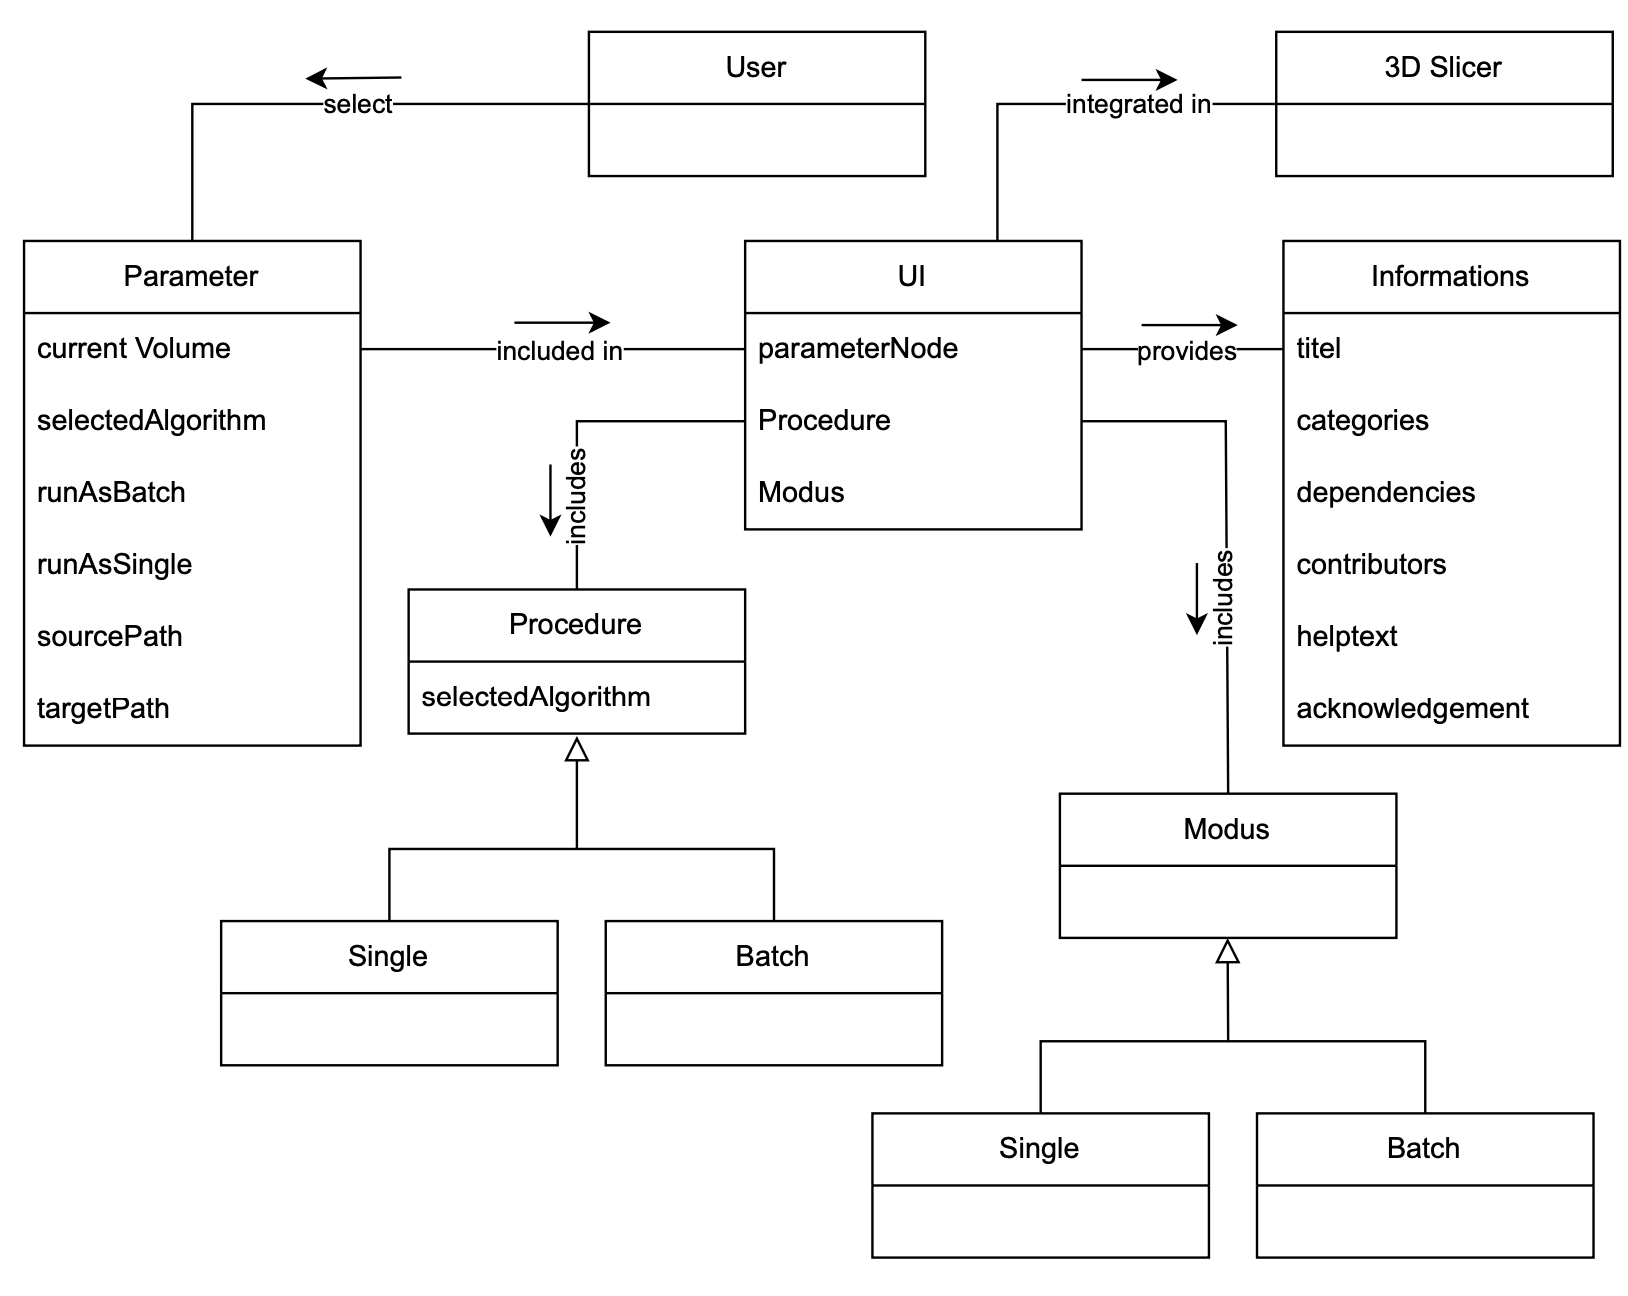
\includegraphics[width=0.75\textwidth]{img/domaenenmodell.jpg}
	\caption{UML-Domänenmodell des gesamten Softwaresystems}
	\label{fig:3d_slicer_domäne}
\end{figure}

Diese doch breite Palette an Anforderungen lässt sich unmöglich auf einmal
bearbeiten. Auch durch eine visuelle Darstellung kann dies nicht vereinfacht werden.
Hierzu sieht diese Arbeit eine Aufteilung in Teilprobleme vor. Der nächste Abschnitt
blickt auf die herausgearbeiteten Anforderungen in diesem Kapitel und leitet daraus
Teilprobleme ab.
% ---------------------------------------------------------------------------------------

\section{Recherche zum Stand der Kunst}
Es ist sehr ungünstig, wenn sich zu Ende eines Projektes herausstellt, dass Lösungen,
in die erhebliche Ressourcen investiert wurden, bereits veröffentlicht sind. Um
dies zu vermeiden, ist eine Umfassende Literaturrecherche nötig, welche den
aktuellen Stand der Technik repräsentiert. Bei der Recherche soll auf Literatur zurückgegriffen
werden, die alle Bereiche abdeckt. Hierbei ist die Rede von Fachliteratur und domänenspezifischen
Literatur. Für dies Arbeit gibt es eine Quelle die von ganz besondere
wichtigkeit ist. die offizielle Dokumentation von \citet{slicer2024}. Diese beinhaltete
gute Anhaltspunkte für die Implementierung. Auch das 3D Slicer Extension Index
ist ein sehr wichtiger Anhaltspunkt, hier bereits erstellte Erweiterungen einsehbar
sind. So kann durch näheres Betrachten andere Module eine Konvention für die
Erstellung einer eigenen Erweiterung abgeleitet werden.
% ---------------------------------------------------------------------------------------

\section{Zerlegung in Teilprobleme}
\label{sec_zerlegung_in_teilprobleme} Durch die Aufteilung des Gesamtsystems in
mehrere kleine Teilaufgaben wird die Software für den Entwicklungsprozess
übersichtlicher. Die einzelnen Domänen können so schneller und besser verstanden
werden. Es gibt viele Möglichkeiten ein Softwaresystem in kleine Teile
aufzuteilen, sodass es am Ende auf den konkreten Anwendungsfall ankommt. Diese
Arbeit sieht folgenden Teilaufgaben für das Gesamtsystem vor:

\begin{itemize}
	\item \textbf{Architekturdesign:} Mithilfe von UML Diagrammen soll die
		Architektur dieses Systems abgebildet werden und sukzessive immer
		detaillierter beschrieben werden. Es soll dann verglichen werden, welche
		Softwarepatterns für dieses System infrage kommen. Durch die Bearbeitung dieses
		Teilproblems kann die Anforderung an eine flexible Architektur erfüllt werden.
		Anschließend kann mit der Entwicklung des UI-Designs begonnen werden.

	\item \textbf{UI Design:} Es soll ein Design erstellt werden, dass sich an erfolgreichen
		und etablierten 3D Slicer Extensions orientiert. Jedoch sollen die Wünsche
		des Endnutzers auch nicht zu kurz kommen. Für eine Visualisierung des Designs
		bedient sich diese Arbeit der Wireframes.

	\item \textbf{Pseudo-Extension:} Bevor der tatsächliche Algorithmus
		eingebunden werden kann, ist es wichtig eine funktionierende Erweiterung zu haben,
		die noch keine konkrete Aufgabe hat, aber funktioniert und in Slicer eingebunden
		werden kann.

	\item \textbf{Hilfsfunktionen:} Nachdem die Infrastruktur der Erweiterung
		steht und funktioniert, kann mit der Implementierung einiger Hilfsfunktionen
		begonnen werden. Hierbei handelt es sich um Methode, die nicht direkt etwas mit
		dem Verfahren zu tun haben, jedoch kleine Nebenaufgaben erfüllen und so
		unumgänglich sind. Als Beispiel sei hier das Laden von CT-Bildern in die Szene
		gedacht.

	\item \textbf{Kappselung Hoffmann:} Nachdem die leere Extension lauffähig ist
		und auch einige Hilfsfunktionen bereitstehen, kann mit der Paketerstellung des
		Hoffmann begonnen werden. Hier soll das Verfahren von einem Python Notebook
		in eine Bibliothek überführt werden, sodass dieses Verfahren in der Extention
		ausführbar ist. Die konkrete Art des Paketes ist noch nicht festgelegt.

	\item \textbf{Speicherung der Parameter:} Der Benutzer steuert das Verfahren
		über die Parameter in der UI. Für die Speicherung der Parametereinstellungen
		hat Slicer den Mechanismus ParameterNode entworfen. Diese wurde bereits in
		Abschnitt \ref{subsec:benutzerschnitstelle} erwähnt. Dieser Mechanismus ist nicht
		trivial, erhöht die Benutzerfreundlichkeit des Systems aber erheblich und
		soll demnach auch in diese Extention Anwendung finden.

	\item \textbf{Single Prozess:} Sobald alle notwendigen Vorbereitungen
		getroffen sind, kann der Algorithmus nun eingebettet werden. Hierzu
		betrachtet man isoliert den Single Prozess. Auch die UI wird erst nur so weit
		entwickel, wie es für den einfachen Prozess nötig ist. Hierbei wird auf das erstellte
		Paket für das Hoffmann Verfahren und die zuvor erstellen Hilfsfunktionen zurückgegriffen.

	\item \textbf{Batch Prozess:} Ist das einfache Verfahren fertig implementiert
		und funktioniert, so kann der Batch Prozess hinzukommen. Hier bedarf es
		einer zusätzlichen Arbeit in der UI, da der Benutzer über das Verwenden dieser
		Funktion gewarnt werden muss. Der Batch Prozess bedarf nämlich erheblicher
		Ressourcen. Hinzukommt die Implementierung einer Fortschrittsanzeige, sodass
		zu erkennen ist, dass ein Hintergrundprozess läuft.

	\item \textbf{Dokumentation und Benutzerhandbuch:} Abschließend ist eine
		ausführliche Dokumentation der Architektur erwünscht, sodass zukünftige Entwickler
		wissen, wo sie ansetzten müssen. Hinzu kommt ein Benutzerhandbuch für eine Verwendung
		der Erweiterung. Das Benutzerhandbuch und die Architekturdokumentation
		erfolgen in einer README.md innerhalb der Extension.

	\item \textbf{Tests:} An letzter Stelle sollen noch Softwaretests
		implementiert werde, um die Richtigkeit der Extension sicherzustellen. 3D
		Slicer sieht hier Unittests vor, die über den Developer Modus in Slicer direkt
		in der jeweiligen Extension ausgeführt werden können.
\end{itemize}

Die Ordnung dieser Punkte gibt eine grobe Orientierung bezüglich der Reihenfolge
während der Umsetzung an. Die wichtigste Aufgabe bei der Umsetzung von
Softwareprojekten ist die ausführliche Recherche zur Findung unterschiedlichster
Lösungsansätze. Nachdem also die Teilaufgaben veststehen, soll der nächste
Abschnitte diese Rechere einleiten und näher beleuchten.
% ---------------------------------------------------------------------------------------

\section{Entwicklungsumgebung}

% ---------------------------------------------------------------------------------------

\section{Forschungsevaluation}
- Evaluationsphase
% ---------------------------------------------------------------------------------------